\documentclass[10pt, a4paper]{article}
\usepackage{lrec2016}
\usepackage[T1]{fontenc}
\usepackage{graphicx}
% for eps graphics

\usepackage{epstopdf}
\usepackage[latin1]{inputenc}

\usepackage{hyperref}
\usepackage{xstring}

\newcommand{\secref}[1]{\StrSubstitute{\getrefnumber{#1}}{.}{ }}

\title{L1ML: Native language identification using TOEFL11}

\name{Yuzhe Chen, Jessica Huynh, Ryan Nicoll}

\address{Brandeis University \\
         Waltham, Massachusetts USA \\
         $\{$yzchen,jhuynh,rnicoll$\}$@brandeis.edu\\}


\abstract{
In this paper, we outline a corpus linguistics-based approach to the task of native language identification (NLI) of L2 writers of English using the TOEFL11 corpus. Previous use of the TOEFL11 corpus for NLI used structural features such as characters, word length, and n-grams for classification features \cite{Tetreault-2013}. To expand upon this research, we provide a description of L1ML, a specification language for annotation of English L2 morphosyntactic errors in noun and verb argument structure and agreement. We demonstrate the utility of this mark-up on a modified gold standard version of the TOEFL11 corpus, where we have provided additional controls for language, question prompt, and score. Finally, we use a Na�ve Bayes classifier to show how the addition of features from L1ML can provide improvement from bare structural features alone. \\ 
\newline 
\Keywords{Native language identification, annotation, English as a second language} }

\begin{document}

\maketitleabstract

\section{Introduction}
In an increasingly interconnected world, languages spoken on a global scale, such as English, have a large number of non-native (NN) speakers who demonstrate systematic linguistic errors in their English in the process of acquiring the language as an adult. Given research that these errors may be dependent on their first language, or L1 \cite{Tetreault-2013}, we set out to show that it may be possible to automatically identify the L1 of these writers from the language-specific errors that they make. 

The study of native language identification (NLI) has been a recently growing area of interest in the field of natural language processing. It has potential applications in a wide variety of fields, including international security, data mining/advertising, second language learning, automatic error correction, among many others.

The L1ML group seeks to capitalize on the errors of NN writers of English through additional annotation following the L1ML, a mark-up language that encodes errors in spelling, punctuation use, and in agreement among nouns, verbs, and other predicates and their corresponding determiners and prepositions. Specifically, we aim to suggest that the addition of annotation can provide robust, salient information that can improve on existing structural features.

\section{Related Work}

\section{Experimental Setup}

\subsection{Corpus}
We have used the TOEFL11 corpus compiled by the Educational Testing Service for our research with some modifications to control for additional variables in testing and a reduction in the universe of languages (which we will called modified TOEFL7, or M-TOEFL7). The TOEFL, or Test of English as a Foreign Language, is an entrance examination akin to the SAT that measures the academic English ability of NN English speakers who wish to enter American universities. 

The original TOEFL11 corpus is comprised of 12,100 open-response unstructured written answers from 11 different languages to 8 general, non-domain specific questions, such as: Do you agree or disagree with the following statement? Young people nowadays do not give enough time to helping their communities. Use specific reasons and examples to support your answer. Each essay is given a score from a low 0 to a high of 5 from three raters, which is then synthesized to produce a global essay score \cite{toefl11-report}. 

This corpus has several useful characteristics that make it especially applicable for this purpose. Perhaps the most important is that it has a wide variety of NN speakers from various L1s (whose L1s are already classified and encoded in the metadata) who are performing a standardized task. Previous researchers have noted the difficulty of compiling such a corpus and the paucity of data available for NLI research that allows for cross-L1 NLI classification \cite{toefl11-report}. Additionally, the TOEFL11 controls for language and prompt by taking a relatively even sampling per language and per prompt. However, it does not currently control for global essay score; consequently, the L1ML team set to modify the corpus to control for score and account for other variables salient to our markup goals. 

For the M-TOEFL7 corpus, we have reduced the universe of languages from 11 to 7 languages: Arabic, Chinese, French, Hindi, Japanese, Telugu, and Spanish. This reduction was instituted in order to provide sufficient time for our volunteer annotators to be able to produce enough data to train our machine learning models (though see discussion in Section 5 for why may not have been as effective as it could be along with possible solutions). These languages were also chosen for their relative difficulty in distinguishing among them for a Na�ve Bayes classifier baseline across the modified version of our corpus (see Section~\ref{sec:ml-baseline} for relevant tables and discussion).

M-TOEFL7 also limited the scope of English proficiency relevant to our current task. In addition to the global essay scores mentioned above, the original compilers of the TOEFL11 corpus categorized each essay into 3 proficiency scores: Low (0--2.5), Medium (2.5--3.5), and High (3.5--5.0). In initial analyses of the data, the L1ML team came to two conclusions. First, the essays in the High categories were virtually indistinguishable from native speaker essays, apart from perhaps one or two small, questionable errors that the three researchers often themselves could not come to agreement on. Second, the Low essays often were short, off-task, and filled with enormous amounts of errors. Part of our annotation task is for our annotators to annotate their corrections (i.e., ``repair'' the errors in the sentence). ``Repair'' as a concept will be discussed more in-depth in Section~\ref{sec:annotation}, but suffice it to say here that it requires that the annotators have a model of what the ``intended'' grammatical sentence of the NN writer was. One of the difficulties the L1ML group encountered was that no standard agreement could be found among what the intended utterance was for most of the sentences in the Low category, given that many of the sentences were semantically/pragmatically bizarre or unmeaningful. 

Given these observations, the L1ML group narrowed the purview of English proficiency to Medium scores, which during initial annotation rounds seemed to have a task-significant number of errors while still allowing annotators to come to agreement on intended utterances for the task. Controlling for score, question prompt, and language, our final M-TOEFL7 corpus ended up with 16 documents for each of Arabic, French, Spanish, Chinese, Japanese, and Hind and 10 documents for Telugu (this last quirk is a product of annotator difficulty---see Section~\ref{sec:annotation} for further discussion). As above, this number of documents was chosen to accommodate our annotators? schedules to provide enough time for our annotators to produce accurate, comprehensive annotations (see Section~\ref{sec:discussion} for discussion on improvements to this process).


\subsection{Annotation\label{sec:annotation}}

Three annotators served as volunteers for our project. Annotators were MA candidates in Computational Linguistics enrolled in COSI 140: Natural Language Annotation for Machine Learning. Annotators had three weeks to annotate approximately 112 documents (16 documents for each of 7 languages) after a first week of annotation where major changes were made to the annotation specification and overall annotation process. The number of annotators was reduced to two due to major illness on the part of one of one annotator.

Each annotator was provided with 2 to 3 languages per week, each separated into a folder of 16 documents delineated by the L1 of the writer. Annotators were also provided with copies of each of the 8 prompts, the annotation specification/guidelines, a copy of the .dtd file to load extent and link tags, and access to the L1ML group Dropbox and GitHub repositories. 
Annotators were initially briefed on the initial specification during a meeting of COSI 140. However, this specification and certain key conventions changed somewhat from the first week of data processing (see discussion in Section~\ref{sec:discussion} for how this may have impacted our data collection scheme/results). 



\subsection{Adjudication and Gold Standard}

\section{Results}

\subsection{Inter-Annotator Agreement}

\subsection{Feature Extraction}

\subsection{Machine Learning Baseline\label{sec:ml-baseline}}
In Table~\ref{table:baseline}, 

\begin{table}[!h]
	\begin{center}
		\begin{tabular}{r|c|c|c|c|c|c|c}	
			\multicolumn{8}{c}{\textbf{Confusion matrix}}\\
			~&ara & fra & hin & jpn & spa & tel & zho\\
			\hline
			ara & <.> & 1 & . & . & 1 & . & . \\
			fra & . & <.> & . & . & . & . & . \\
			hin & . & 1 & <.> & . & . & . & . \\
			jpn & 1 & . & . & <1> & . & . & . \\
			spa & . & . & 1 & . & <.> & . & . \\
			tel & . & 1 & 2 & 2 & 2 & <2> & 3 \\
			zho & 2 & . & . & . & . & . & <.> \\
			
			\multicolumn{8}{c}{\textbf{Measures}}\\
			ara & \multicolumn{4}{l}{\textit{Precision}: 0.000} & \multicolumn{3}{l}{\textit{Recall}: 0.000}	\\
			fra & \multicolumn{4}{l}{\textit{Precision}: ---} & \multicolumn{3}{l}{\textit{Recall}: 0.000}	\\
			hin & \multicolumn{4}{l}{\textit{Precision}: 0.000} & \multicolumn{3}{l}{\textit{Recall}: 0.000}	\\
			jpn & \multicolumn{4}{l}{\textit{Precision}: 0.500} & \multicolumn{3}{l}{\textit{Recall}: 0.333}	\\
			spa & \multicolumn{4}{l}{\textit{Precision}: 0.000} & \multicolumn{3}{l}{\textit{Recall}: 0.000}	\\
			tel & \multicolumn{4}{l}{\textit{Precision}: 0.167} & \multicolumn{3}{l}{\textit{Recall}: 1.000}	\\
			zho & \multicolumn{4}{l}{\textit{Precision}: 0.000} & \multicolumn{3}{l}{\textit{Recall}: 0.000}	\\
			\multicolumn{4}{c}{\textit{Accuracy}: 0.150} & \multicolumn{4}{l}{\textit{Macro-averaged }$F_1$: 0.127} 
		\end{tabular}
		\caption{Baseline classifier using 106 documents, omitting annotations and names of countries and places\label{table:baseline}}
	\end{center}
\end{table}

\subsection{Most Salient Features}

\section{Discussion and Conclusion\label{sec:discussion}}

\section{Paper}

Each manuscript should be submitted on white \textbf{A4 paper.} The fully
justified text should be formatted in two parallel columns, each 8.25 cm wide,
and separated by a space of 0.63 cm. Left, right, and bottom margins should be
1.9 cm. and the top margin 2.5 cm. The font for the main body of the text should
be Times 10 pt with interlinear spacing of 12 pt.  \textbf{Articles must be
between 4 and 8 pages in length}, regardless of the mode of presentation (oral
or poster).

\section{General Instructions}

Each paper is allocated between \underline{\textbf{a mi\-ni\-mum of four}}
\textbf{\underline{and a maximum of eight pages}} including figures. %\newline

The unprotected PDF files will appear in the on-line proceedings directly as
received. Do not print the page number.

\section{Page Numbering}

\textbf{Please do not include page numbers in your article.} The definitive page
numbering of articles published in the proceedings will be decided by the
organizing committee.

\section{Headings / Level 1 Headings}

Headings should be capitalised in the same way as the main title, and centred
within the column. The font used is Times 12 bold. There should also be a space
of 12 pt between the title and the preceding section, and a space of 3 pt
between the title and the text following it.

\subsection{Level 2 Headings}

The format for level 2 headings is the same as for level 1 Headings, with the
font Times 11, and the heading is justified to the left of the column.

\subsubsection{Level 3 Headings}

The format for level 3 headings is the same as for level 2 headings, except that
the font is Times 10, and there should be no space left between the heading and
the text.

%\subsubsection{Example of a sub-subsection with a long heading that will occupy two lines}
%
%Yet another example of a sub-subsection. Yet another example of a sub-subsection. Yet another example of a sub-subsection. Yet another example of a sub-subsection. Yet another example of a sub-subsection.

\section{Citing References in the Text}

\subsection{Bibliographical References}

All bibliographical references within the text should be placed in parentheses
containing the author's surname followed by a comma before the date of
publication \cite{Martin-90}. If the sentence already includes the author's
name, then it is only necessary to put the date in parentheses:
\newcite{Martin-90}. When several authors are cited, those references should be
separated with a semicolon: \cite{Martin-90,CastorPollux-92}. When the reference
has more than three authors, only cite the name of the first author followed by
et al. (e.g. \cite{Superman-Batman-Catwoman-Spiderman-00}).


\subsubsection{When Not Citing Any Language Resource}

When no language resource needs to be cited in the paper, you need to comment
out a few lines in the \texttt{.tex} file:

\begin{verbatim}
% \usepackage{multibib}
% \newcites{languageresource}{}
% \section{Language Resource References}
% \bibliographystylelanguageresource
%   {lrec2016}
% \bibliographylanguageresource{xample}
\end{verbatim}

\section{Figures \& Tables}
\subsection{Figures}

All figures should be centred and clearly distinguishable. They should never be
drawn by hand, and the lines must be very dark in order to ensure a high-quality
printed version. Figures should be numbered in the text, and have a caption in
Times 10 pt underneath. A space must be left between each figure and its
respective caption. 

Example of a figure enclosed in a box:

\begin{figure}[!h]
\begin{center}
%\fbox{\parbox{6cm}{
%This is a figure with a caption.}}
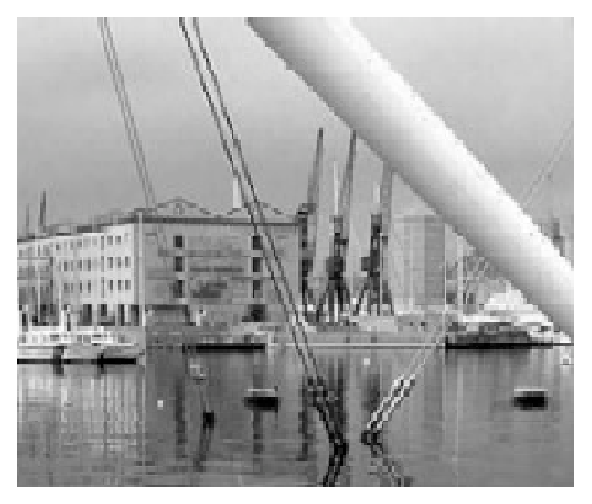
\includegraphics[scale=0.5]{image1.eps} 
\caption{The caption of the figure.}
\label{fig.1}
\end{center}
\end{figure}

Figure and caption should always appear together on the same page. Large figures
can be centred, using a full page.
%NB: an example of large figures is missing.  \newpage

\subsection{Tables}

The instructions for tables are the same as for figures.
%Two types of tables are distinguished: in-column and big tables that don't fit in the columns.
%\subsection{In-column tables}
%An example of an in-column table is presented here.
%
\begin{table}[!h]
\begin{center}
\begin{tabular}{|l|l|}

      \hline
      Level&Tools\\
      \hline\hline
      Morphology & Pitrat Analyser\\
      Syntax & LFG Analyser (C-Structure)\\
     % Semantics & LFG F-Structures + Sowa's\\
     % & Conceptual Graphs\\
      \hline

\end{tabular}
\caption{The caption of the table}
 \end{center}
\end{table}

%\subsection{Big tables}
%
%An example of a big table which extends beyond the column and will
%float in the next page.
%
% \begin{table*}[ht]
% \begin{center}
% \begin{tabular}{|l|l|}
%
%       \hline
%       Level&Tools\\
%       \hline\hline
%       Morphology & Pitrat Analyser\\
%       Syntax & LFG Analyser (C-Structure)\\
%       Semantics & LFG F-Structures + Sowa's Conceptual Graphs  \\
%       \hline
%
% \end{tabular}
% \caption{The caption of the big table}
% \end{center}
% \end{table*}
%

\section{Footnotes}

Footnotes are indicated within the text by a number in superscript\footnote{They
should be in Times 9, and appear at the bottom of the same page as their
corresponding number. Footnotes should also be separated from the rest of the
text by a horizontal line 5 cm long.}.

\section{Copyrights}

The The Lan\-gua\-ge Re\-sour\-ce and Evalua\-tion Con\-fe\-rence (LREC)
proceedings are published by the European Language Resources Association (ELRA).
They are available online from the conference website.


ELRA's policy is to acquire copyright for all LREC contributions. In assigning
your copyright, you are not forfeiting your right to use your contribution
elsewhere. This you may do without seeking permission and is subject only to
normal acknowledgement to the LREC proceedings. The LREC 2016 Proceedings are
licensed under CC-BY-NC, the Creative Commons Attribution-NonCommercial 4.0
International License.

\section{Conclusion}

Your submission of a finalized contribution for inclusion in the LREC
proceedings automatically assigns the above-mentioned copyright to ELRA.


\section{Acknowledgements}

Place all acknowledgements (including those concerning research grants and
funding) in a separate section at the end of the article.

\section{Providing References}

\subsection{Bibliographical References}
Bibliographical references should be listed in alphabetical order at the
end of the article. The title of the section, ``Bibliographical References'',
should be a level 1 heading. The first line of each bibliographical reference
should be justified to the left of the column, and the rest of the entry should
be indented by 0.35 cm.

The examples provided in Section \secref{main:ref} (some of which are fictitious
references) illustrate the basic format required for articles in conference
proceedings, books, journals articles, Ph.D. theses, and chapters of books.

\subsection{Language Resource References}

Language resource references should be listed in alphabetical order at the end
of the article, in the ``Language Resource References'' section, placed after
the ``Bibliographical References'' section. The title of the ``Language Resource
References'' section, should be a level 1 heading. The first line of each
language resource reference should be justified to the left of the column, and
the rest of the entry should be indented by 0.35 cm. The example in Section 
\secref{lr:ref} illustrates the basic format required for language resources.

In order to be able to cite a language resource, it must be added to
the \texttt{.bib} file first, as a \texttt{@LanguageResource} item type, which
contains the following fields:

\begin{itemize}
    \item{\texttt{author}: the builder of the resource}
    \item{\texttt{title}: the name of the resource}
    \item{\texttt{publisher}: the publisher of the resource (project,
          organization etc)}
    \item{\texttt{year}: year of the resource release}
    \item{\texttt{series}: more general resource set this language resource
          belongs to}
    \item{\texttt{edition}: version of the resource}
    \item{\texttt{islrn}: the International Standard Language Resource Number
          (ISLRN) of the resource\footnote{The ISLRN number is available from
          \texttt{http://islrn.org}}} 
\end{itemize}

If you want the full resource author name to appear in the citation, the
language resource author name should be protected by enclosing it between
\texttt{\{...\}}, as shown in the model \texttt{.bib} file.

\section*{Appendix: How to Produce the \texttt{.pdf} Version}

In order to generate a PDF file out of the LaTeX file herein, when citing
language resources, the following steps need to be performed:

\begin{itemize}
    \item{Compile the \texttt{.tex} file once}
    \item{Invoke \texttt{bibtex} on the eponymous \texttt{.aux} file}
    \item{Invoke \texttt{bibtex} on the \texttt{languageresources.aux} file}
    \item{Compile the \texttt{.tex} file twice}
\end{itemize}

% \nocite{*}
\section{Bibliographical References}
\label{main:ref}

\bibliographystyle{lrec2016}
\bibliography{l1ml-final}


\end{document}
